\subsection{Representativeness}
\label{sec:rep}

We begin by analyzing the default representativeness of LMs,  at an overall (\emph{does its opinion distribution match that of the overall US populace?}) and group level (\emph{does it match a particular group's opinion?}).
To measure this, we evaluate model opinion distribution on \bname questions \emph{without} any context (beyond the question itself).

\paragraph{The metric.} We define the representativeness of an LM with respect to the overall population as the average alignment (Section~\ref{sec:metric})---across questions---between the default opinion distribution of the model and that of the overall population, \ie, 
\begin{equation}
    \mathcal{R}^{O}_m(Q) = \simi(D_m, D_O, Q).
  \end{equation}

Analogously, we can define the group representativeness of an LM w.r.t. to a particular demographic group $G$ as $\mathcal{R}^G_m(Q) := \simi(D_m, D_G, Q)$.
A higher overall (group) representativeness score indicates that out-of-the-box, the LM is better aligned with the distribution of viewpoints held by the overall US populace (that group).
While the maximum possible of this score is 1, it cannot be achieved for \emph{all} of the groups.
This is due to the fact that there are irreconcilable differences between the opinions of certain groups (\eg, Democrats and Republicans on guns in Figure~\ref{fig:prompt_example})---making it impossible for the model's opinion distribution $D_m$ to simultaneously match all of them.



\paragraph{Are current LMs representative?}
Figure~\ref{fig:alignment_basic} depicts the overall representativeness scores $\mathcal{R}^{O}_m$ of different LMs.
Overall, we observe that none of the models are perfectly representative of the general populace (of survey respondents).
In fact, more recent models trained to be more human-aligned~\citep{ouyang2022training,ai21instructbeta} are actually \emph{worse}---cf. OpenAI's \model{text-davinci-003} and \model{davinci} models.
To put these results into context, we compare them to salient human baselines:
\begin{itemize}
  \item First, we consider the alignment between the opinions of a each of our 60 demographic groups and the general populace ($\mathcal{R}^{O}_{G}(Q) = \simi(D_{G}, D_O, Q)$). We see that every one of these groups is \emph{more} representative of the overall populace than \emph{any} of the LMs we consider (i.e., cf. representativeness scores of `human (worst)` to all the LMs).
  \item Second, we construct a scale of alignment values between pairs of demographic groups on questions from specific contentious topics ($\mathcal{R}^{G_1}_{G_2}(Q_T) = \simi(D_{G_1}, D_{G_2}, Q_T)$). On this scale, we see that $\mathcal{R}^{O}_m$ for most models is comparable to the opinion alignment of agnostic and orthodox people on abortion or Democrats and Republicans on climate change.
\end{itemize}


\begin{figure}[!t]
    \vskip 0.2in
    \begin{center}
      \begin{subfigure}[b]{0.47\textwidth}
        \centering
        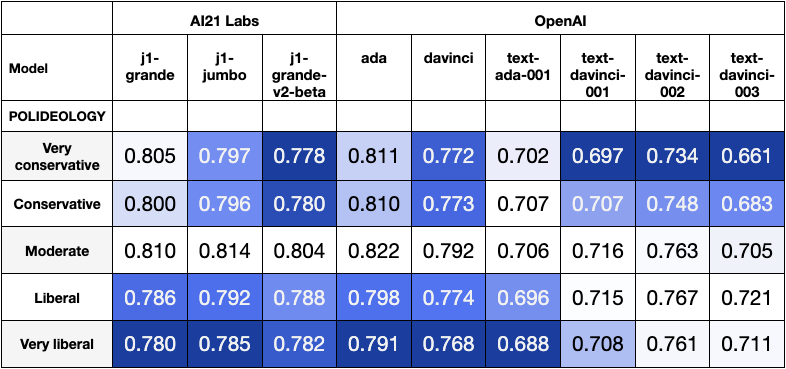
\includegraphics[width=1\columnwidth]{Figures/representativeness_POLIDEOLOGY.png}
      \end{subfigure} \hfil
      \begin{subfigure}[b]{0.485\textwidth}
        \centering
        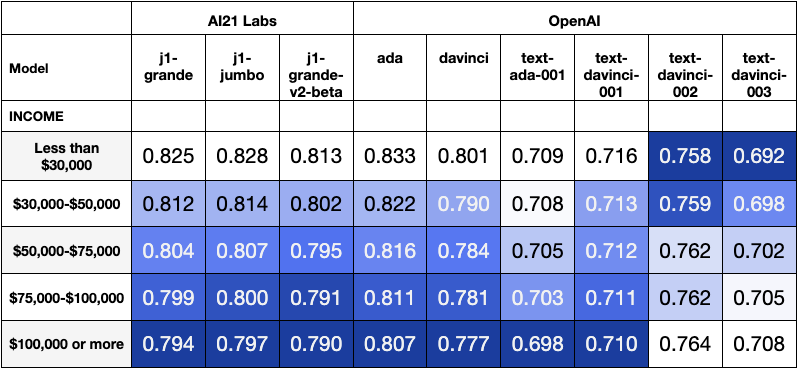
\includegraphics[width=1\columnwidth]{Figures/representativeness_INCOME.png}
      \end{subfigure}
    \caption{Group representativeness scores $\mathcal{R}^{G}_m$ of LMs as a function of political ideology and income: A higher score (lighter) indicates that, on average across dataset questions, the LMs opinion distribution is more similar to that of survey respondents from the specified group (\ie, $\mathcal{R}^G_m(Q)$ is larger). The coloring is normalized by column to highlight the groups a given model (column) is most/least aligned to. We find that the demographic groups with the highest representativeness shift from base LM (moderate to conservative with low income) to the RLHF trained ones (liberal and high income). Other demographic categories are shown in Appendix~\ref{figapp:per_md_alignment}.
      }
    \label{fig:per_md_alignment}
    \end{center}
    \vskip -0.2in
\end{figure}


\paragraph{Group representativeness.} The group representativeness scores for all the base LMs share striking similarities---\eg, being most aligned with lower income, moderate, and Protestant or Roman Catholic groups. 
This might be because all these models were trained on  snapshots of the internet---and thus mimic similar pools of human writers.
While AI21's HF-tuned model (\texttt{j1-grande-v2-beta}) behaves similarly to base LMs, the corresponding OpenAI instruct series models (\texttt{text-*}) are markedly different.
The opinions reflected by these models align more with people who are liberal, high income, well-educated, and not religious or belong to religions other than Buddhists, Muslims, and Hindus.
These groups line up with the demographics of the crowd-workers reported in OpenAI's InstructGPT paper~\citep{ouyang2022training}---\eg, predominantly young Southeast Asian and White with a college degree\footnote{While our results agree with the crowdworker demographics in the instructGPT paper, we cannot draw the conclusion that our approach recovers the RLHF crowdworker distribution, as the datasets and crowdworkers used in OpenAI's production systems are not public.}.
Finally, a broader analysis across all the groups in the Pew survey highlights several that have low representativeness scores for all LMs, such as individuals of age 65+, widowed, and high religious attendance (Appendix~\ref{figapp:per_md_alignment}). In the case of age, the InstructGPT paper similarly shows that there were almost no individuals of age 65+ that were part of the crowdsourcing process, and it is likely that the other groups (widowed, high religious attendance) may also be difficult to recruit through standard crowdsourcing vendors.


\begin{figure}[!t]
    \vskip 0.2in
    \begin{center}
      \begin{subfigure}[b]{0.45\textwidth}
        \centering
        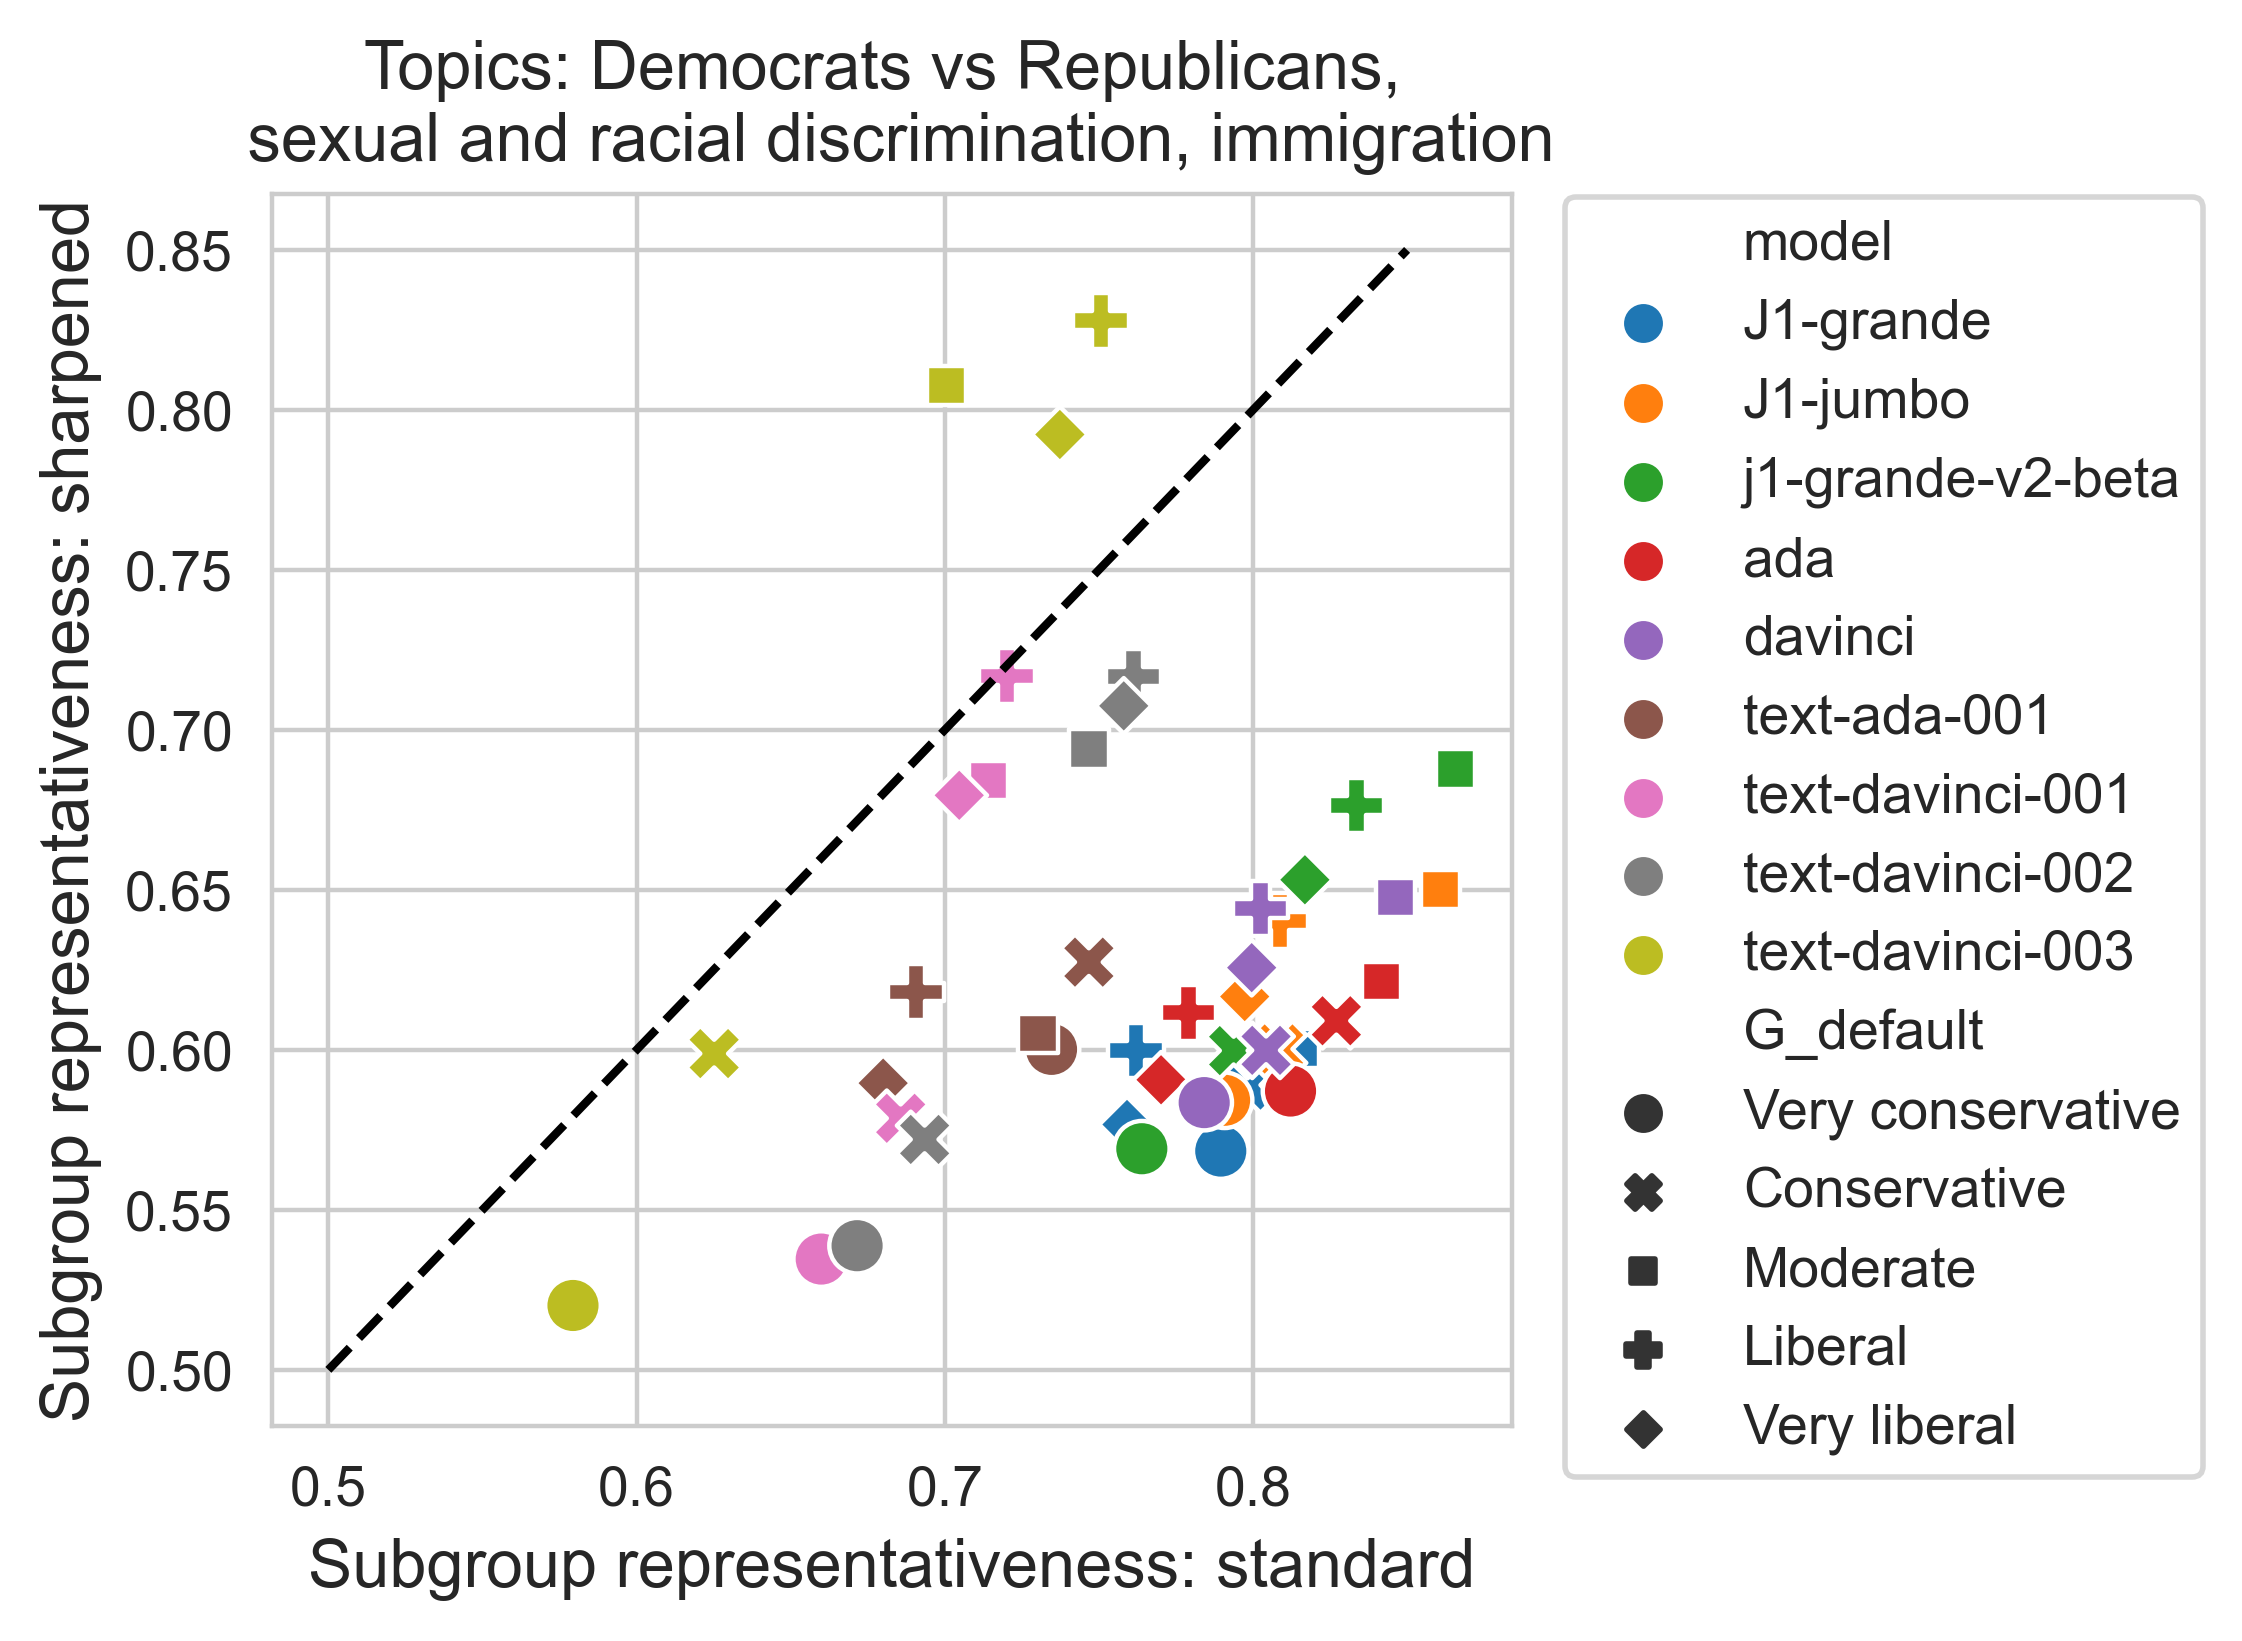
\includegraphics[width=1\columnwidth]{Figures/caricature.png}
        \caption{}
        \label{fig:polarized_alignment}
      \end{subfigure} \hfil
      \begin{subfigure}[b]{0.48\textwidth}
        \centering
        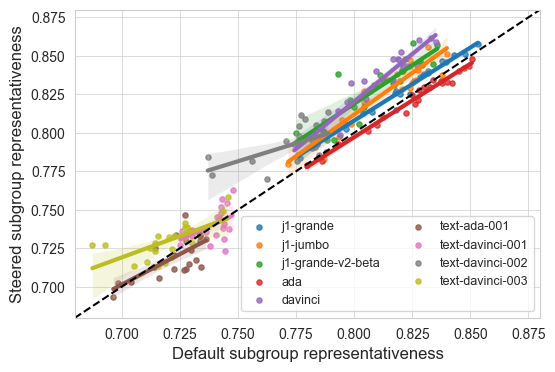
\includegraphics[width=1\columnwidth]{Figures/steerability.png}
        \caption{}
        \label{fig:steerability_overall}
      \end{subfigure} 
    \end{center}
    \caption{(a) The alignment of LM opinions with the actual and modal views of different ideological groups on contentious topics. (b) Steerability of LMs towards specific demographic groups: we compare the group representativeness of models by default (x-axis, $\mathcal{R}^G_m$) and with steering $\steer^G_m$ (y-axis). Each point represents a choice of model $m$ and target group $G$, and points above the $x=y$ line indicate pairs where the model's opinion alignment improves under steering. Shaded lines indicate linear trends for each model $m$, and we generally observe that models improve from steering (above $x=y$) but the amount of improvement is limited.}
    \vskip -0.2in
\end{figure}


\paragraph{Modal representativeness.}
\label{sec:polarization}
In Figures~\ref{fig:alignment_basic} and~\ref{fig:per_md_alignment}, we saw that human-feedback tuned models (and most notably \model{text-davinci-003}) are \emph{less representative} of overall opinions.
A closer look at \texttt{text-davinci-003}'s opinion distribution provides some insight into why this might be the case.
Specifically, it has an extremely sharp (and low entropy) opinion distribution for most questions (Appendix Figure~\ref{figapp:entropy})---it typically assigns $>0.99$ probability to one of the options.
This is unlike humans, who even on contentious topics (like gun rights), tend to exhibit some diversity in opinions (see the Democratic respondent distribution in Figure~\ref{fig:prompt_example}).
This prompts us to ask: is \texttt{text-davinci-003} actually unrepresentative, or does it collapse to the most-frequent and \emph{modal} opinion of certain groups?
To test this, we construct a ``modal'' opinion distribution of a group by applying temperature scaling to the group's opinion distribution $D_G(q)$ (Appendix~\ref{app:temp}).
In Figure~\ref{fig:polarized_alignment}, we then compare the relative tendencies of LMs to match the actual and modal opinions of different political groups on contentious topics.


We observe that the behavior of \model{text-davinci-003} is quite unique: its opinion distribution seems to converge to the modal views of liberals and moderates.
This indicates that the dominant approach of aligning LMs with RL based human-feedback not only skews the model's opinions towards certain groups (liberals), but also pushes the model to almost embody caricatures of those groups (\eg, 99\% approval of Joe Biden).
From a different standpoint, this finding highlights the importance of considering the entire spectrum of human responses rather than just the mode. A modal analysis of \texttt{text-davinci-003} would conclude that the model is highly representative of Democrats, where in reality its representation collapses the diversity of opinions held by different democrats into a single, modal response.

\paragraph{Refusals.}
In our comparison of human and LM opinions so far, we omitted the ``refusal'' option for all questions due to its non-ordinal nature.
In Appendix~\ref{app:refusal}, we thus separately compare the refusal rates of LMs and human respondents. 
We find that all models have low refusal rates. 
Although human feedback-tuned models are encouraged to refuse to take a stance on contentious issues~\citep{askell2021general,ouyang2022training}, they tend to rarely do so in our multiple-choice setting---with refusal rates as low as 1--2\%.